\documentclass[./../../paper.tex]{subfiles}
\graphicspath{{\subfix{./../../figures/}}}

\begin{document}
% TODO: search for paper 
In this thesis, we approach the problem of generating counterfactuals for processes. The literature has provided a multitude of techniques to generate counterfactuals for AI models, that are derived from static data\footnote{With static data, we refer to data that does not change over a time dimension.}. However, little research has focussed on counterfactuals for dynamic data\footnote{With dynamic data, we refer to data that has a temporal relationship as a major component, which is also inherently sequential}.  

For process data, the literature often uses terms like structured and semi-structured, as they are related to the staticity and dynamicity. Both, structuredness and semi-structuredness, often relate to the data model, in which we structure the information at hand. 
As static data neither changes over time nor changes its structure, we can use structured data-formats such as tables to capture the information where each data point is an independent entity. We can take the MNIST dataset\cite{deng_MNISTDatabaseHandwritten_2012} or Iris dataset\cite{anderson_SpeciesProblemIris_1936,fisher_UseMultipleMeasurements_1936} as examples for structured and static data. 
In both datasets, all data points are independent and have the same amount of attributes. In contrast, semi-structured data does not have to follow these strict characteristics. Here, data points often belong to a group of data points which constitutes the full entity. Furthermore, the attributes of each data point may vary. The grouping mechanism could take the form of associative links, class associations or temporal cause-effect relationships. Examples of these are Part-of-Speech datasets like Penn Treebank set\cite{marcus_Buildinglargeannotated_1993}. 
Here, we often associate each data point with a sentence. However, the temporal relationship between words is debatable and hence, whether the data is \emph{dynamic}, as well. So, not all semi-structured datasets are dynamic and vice versa. However, structured data will almost always be static, with the exception of time-series. 
Lastly, there is also unstructured data, which does not incorporate any specific data model. Corpora like the Brown dataset\cite{francis79browncorpus}, for instance, are collections of text heavy unstructured information. In \autoref{fig:example_structure}, we show various examples of data.


\begin{figure}
    \centering
    \begin{subfigure}[c]{0.49\textwidth}
        \centering
        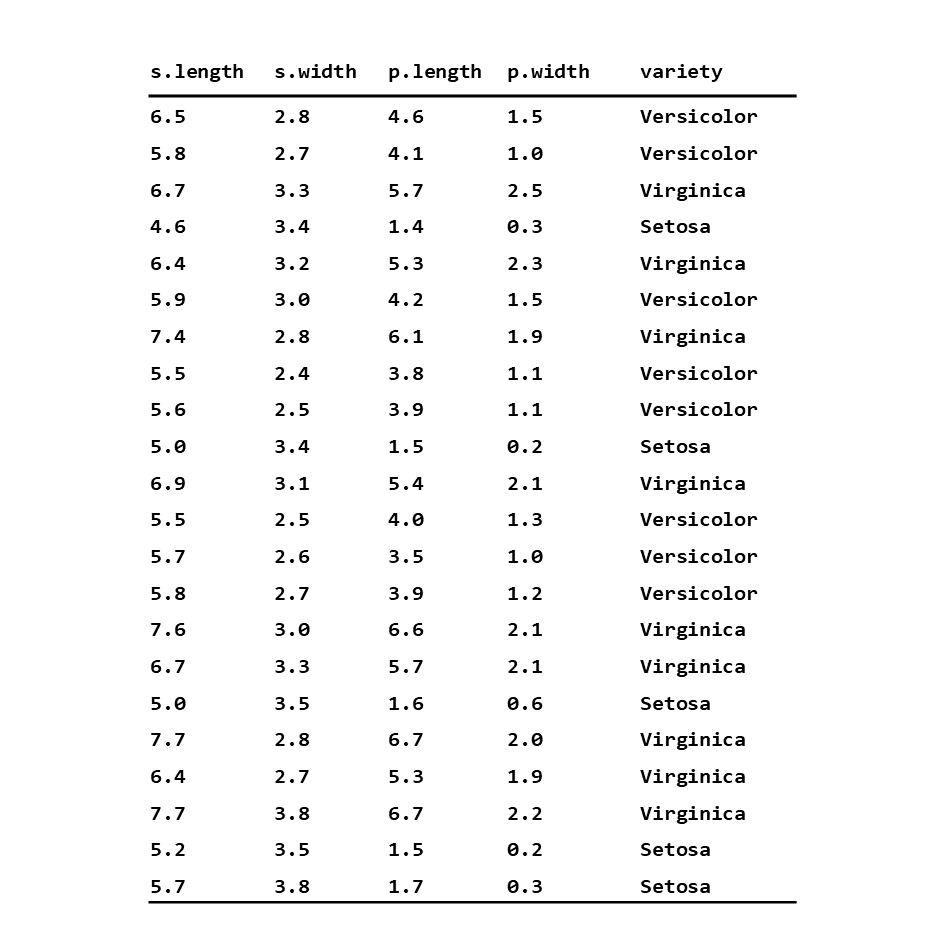
\includegraphics[width=\textwidth]{figures/Graphics/Slide1.png}
        \caption{An excerpt of the MNIST dataset. This is a structured dataset.}
        \label{fig:structured}
    \end{subfigure}
    \hfill
    \begin{subfigure}[c]{0.49\textwidth}
        \centering
        
\includegraphics[width=\textwidth]{figures/Graphics/Slide3.png}
        \caption{A number of heterogenous documents. A dataset like this is unstructured.}
        \label{fig:unstructured}
    \end{subfigure}
    \hfill
    \begin{subfigure}[c]{0.7\textwidth}
        \centering
        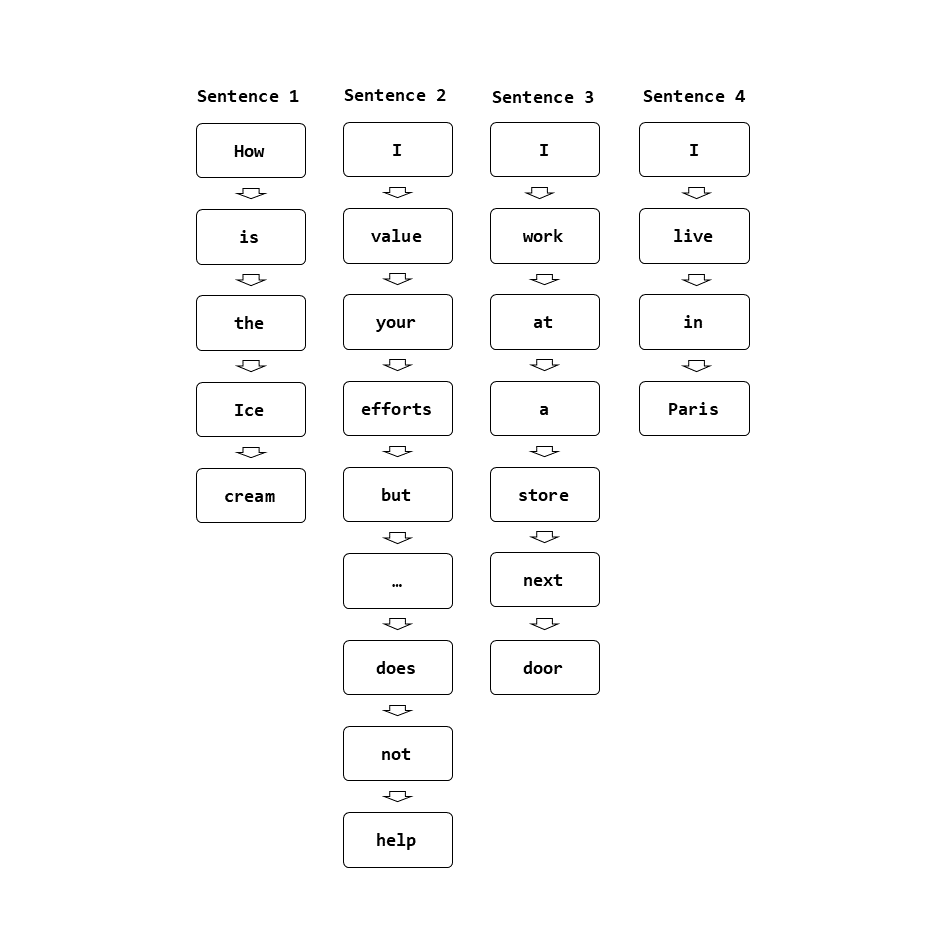
\includegraphics[width=\textwidth]{figures/Graphics/Slide2.png}
        \caption{Multiple seqeuences of words. Each word forms a sentence of different lengths. Therefore, this data is semi-structured.}
        \label{fig:semistructured}
    \end{subfigure}
       \caption{Schematic examples of static structured, dynamic semi-structured data and unstructured data.}
       \label{fig:example_structure}
\end{figure}


A major reason, why there has not been much research on counterfactuals for dynamic semi-structured data, emerges from a multitude of challenges, when dealing with counterfactuals and sequences. Three of these challenges are particularly important.
 
First, counterfactuals within AI attempt to explain outcomes which never occured. \emph{What-if} questions often refer to hypothetical scenarios. Therefore, there is no evidential data from which we can infer predictions. Subsequently, this lack of evidence further complicates the evaluation of generated counterfactuals. In other words, you cannot validate the correctness of a theoretical outcome that has never occured.

Second, sequential data is highly variable in length, but process steps have complicated factors, too. The sequential nature of the data impedes the tractability of many problems due to the combinatorial explosion of possible sequences. 
%A sequence with 10 possible elements at each position will have a 100, 1000 and 10.000 possible combinations, if they have a sequence length of 2, 3 and 4, respectively. 
Furthermore, the data generated is seldomly one-dimensional or discrete. Henceforth, each dimension's contribution can vary in dependance of its context, time and magnitude. 
%Each element in a sequence can have additional information attached to it.

Third, process data often requires knowledge of the causal structures that produced the data in the first place. However, these structures are often hidden and it is a NP-hard problem to elicit them\cite{wang_Efficientrecoverymissing_2013}.

These challenges make the field, in which we can contribute, a vast endeavor. 

\end{document}
